\section{Conscious Participation in World Events}

\begin{quotex}
Wisdom has built her house, she has set up her seven pillars.
\flright{\textit{Proverbs 9:1}}

\end{quotex}

The Bateleur represents Unity, which transcends thought, desire, volition, that is, the entire world process. It
represents Intuition, mystical awareness, or a cognition beyond discursive thought. This ``first act of intelligence" is
a gift of the Spirit, who blows he wills, so it is not the customary way we know.

In ordinary life, to know is to be conscious of something, so duality arises, represented by the High Priestess. This
``other" is the reflection of Spirit, represented by Water. This is the feminine principle, the \textbf{Divine Sophia},
which builds the house of Being. Thus, everything in the world of form is actually the symbol or ``signature" of
Transcendence, in the words of Schwaller de Lubicz.

\begin{wrapfigure}{rt}{.2\textwidth}
 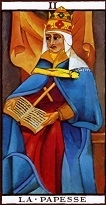
\includegraphics[scale=5]{a20101015ConsciousParticipationinWorldEvents-img001.jpg}
\end{wrapfigure} 

The Transcendent takes form both in the subtle and gross realms of manifestation. The gross realm includes all existing
things we experience. But initially, it reveals itself as thoughts in the subtle realm. This card shows us the
connection between these two realms.

In everyday life, we stop at the thought, treating it as an end in itself. We have no concern as to its origin or its
deeper meaning. It is meditation that leads us to depth. Valentin Tomberg writes in \emph{New Testament Studies}:

\begin{quotex}
It is very difficult in our time to distinguish between thinking of something and meditating on it. This is especially
difficult because, while meditation arises as the result of deep thinking, from a certain perspective meditation not
only differs from thinking, but it is actually the opposite. … meditation involves repeated submersion into the
insight.

\end{quotex}
So what happens when we meditate?

\begin{quotex}
The purpose of meditation is not to gain new knowledge, but to live in acquired knowledge. The discovery of new thought
content is not the goal of meditation: the object is to bring thought content down into the life of feeling and
volition. The goal of meditation is to make a truth the content of one's whole being. And
meditation must be continued for as long as it takes to change clear thought into a clear force of the will.

\end{quotex}
The thought, which is the reflection of the divine idea, must come alive. To do so, it cannot remain dispassionate, but
must enter into our feeling life (also part of subtle manifestation). This activates the Will —
the idea guides the Will and the feeling motivates the Will. The role of the Will, then, is to manifest creatively in
the World Process. This is the formula of manifestation:

Intuition $\Rightarrow $ Thought $\Rightarrow $ Will $\Rightarrow $ Manifestation

Valentin Tomberg puts it this way:

\begin{quotex}
Meditation leads to conscious participation in objective world events.

\end{quotex}


\flrightit{Posted on 2010-10-15 by Cologero }
